\chapter{Experiments}
\label{sec:experiments}

% Zu jeder Arbeit in unserem Bereich gehört eine Leistungsbewertung. Aus
% diesem Kapitel sollte hervorgehen, welche Methoden angewandt worden,
% die Leistungsfähigkeit zu bewerten und welche Ergabnisse dabei erzielt
% wurden. Wichtig ist es, dem Leser nicht nur ein paar Zahlen
% hinzustellen, sondern auch eine Diskussion der Ergebnisse
% vorzunehmen. Es wird empfohlen zunächst die eigenen Erwartungen
% bezüglich der Ergebnisse zu erläutern und anschließend eventuell
% festgestellte Abweichungen zu erklären.

%statistical analysis and signal processing are being increasingly applied to private data obtained from individuals
The DC network from chapter 3 ensures anonymity of user data in a smart grid. It is impossible for an electricity provider to obtain the individual electricity consumption of a user without performing aggressive attacks. But this criterion alone is insufficient. In chapter two, it was described that 52 different household appliances could be correctly identified from the aggregated electricity consumption of two houses with a accuracy of 55\% and a measurement interval of 1 hour\ref{subsec:low_reso}. Accordingly, it is still possible to draw conclusions about individual electricity consumption or about the use of household appliances from different households from an aggregated result. In addition, the measurement interval in the German smart grid is much more frequent and amounts to 15 minutes. Therefore, the DC network must have a minimum number of participants to make an analysis over the aggregated result impossible. For this purpose, an experimental analysis was performed in the master thesis to be able to make a statement about the minimum number of participants in a DC network. When researching the information content of aggregated data, only sparse information and no common metric could be found. In particular, of interest is: How much electricity consumption from individual households needs to be aggregated so that certain characteristics, such as the use of individual household appliances, can no longer be analyzed from the results? In this chapter, the experiment investigates from how many participants in the DC network it can be said with certainty that it is no longer possible to draw conclusions about individual users from the result. For this purpose, the assumption and the structure of the experiment and its execution will be described first. Afterwards the results of the experiment are considered and analyzed.
\\
\\
\textbf{Assumption}
\\
\\
The goal of the experiment is that no inferences can be drawn from the result of the aggregated electricity consumption. This includes that no persons can be deanonymized from the result or that no household appliances can be identified from the result. There is no metric that can measure anonymity from electricity consumption, but there are metrics that can measure the information content of electricity consumption[ref]. The assumption is therefore that if the information content from the aggregated result of electricity consumption is low, then no conclusions can be drawn about individual households or household appliances.
\\
\\
\section{Experimental Setup}
\\
\\
\ref{subsec:information_gain} described which metrics can calculate the information content of aggregated electricity consumptions. For the first experiment, a different procedure was chosen. Electricity consumptions from the London Smart Meter dataset were used[london smart meter]. In the dataset, the electricity consumption of 5,567 different households between 2011 and 2014 were recorded with measurement intervals of 30 minutes each. In the experiment, $N$ houses were selected and their electricity consumptions were aggregated for each time point. From the aggregated result ($ar$) the normalized standard deviation ($nominated\:sd$) for each individual time stamp was calculated and compared to the individual electricity consumption of a house at that time. The comparison looks if the electricity consumption of a single house is within the tolerance limit of the aggregated result. The tolerance limit ($l$) is the following interval:
\begin{equation}
\label{eq:open_commit}
ar- nominated\:sd< l < ar + nominated\:sd
\end{equation}
If the electricity consumption of a house is above or below the tolerance limit at a point in time, then it is assumed that the electricity consumption of the house has a high information content at that point in time and that this information content could be read from the aggregated result. For each time stamp, each house is counted individually for how often the individual power consumptions are outside the tolerance limit. In order to perform the experiment, a script was programmed in R, which selects random houses from the London Smart Meter data set. Additionally, the data set got filtered for houses that have readings between 2013 and 2014. For the highest possible precision of the calculation, it was ensured that when a comparison calculation is performed, the time stamp is also correctly identical. In short every 30 minutes measurements in 2013-2014 of a house were compared whether the electricity consumption is above or below the tolerance limit of the aggregated results of N houses. For each calculation, the number of times the values are outside the tolerance limit is counted. This experiment was repeated with different N sizes to analyze how strong the effects of the information content in the aggregated result are measurable.\\
A second experiment was also executed. This time, not the time span of one year was examined, but the time span of 2 weeks. Due to the shorter time span and the resulting much faster execution of the second experiment, the Kullback Leibler Divergence could additionally be calculated. 
The Kullback Leibler divergence is often referred to as relative entropy and was introduced in \ref{subsec:information_gain}.
The second experiment is carried out essentially like the first experiment. It is counted for one week how often the electricity consumption of one house deviates from the standard deviation of the electricity consumption of $N$ houses. In the second week, another house ($N+1$) is added to the pool of houses already analyzed. It is now analyzed if the added house has a high influence on the overall result and if the added house stands out from the standard deviation of the first week and has especially many deviations. If the added house does not differ from the other houses in terms of deviations, then it can be assumed that new users are added to the DC network without any additional user behavior being noticeable in the result. In addition to the standard deviation as a metric for anonymity, the Kullback Leibler Divergence was calculated for each house in the second experiment. \todo{vllt noch ein bisschen mehr?}
\\
\\
\textbf{Yearly Results}
\\
\\
Figure \ref{img:2_Houses} - \ref{img:150_houses} show the results of the experimental tests where the measured time period is one year. Experiments were conducted with 2, 3, 5, 10, 25, 50, 100 and 150 random chosen houses per group, whose electricity consumptions were aggregated and the experiments were repeated 2 times. The experiments start with a size of 2 houses, because this is the smallest possible DC network. On the X-axis the time in months can be read. On the Y-axis, the average daily electricity consumption within half an hour of a house is shown. If the figure is viewed, it can be seen that in the experiments with little aggregated houses \ref{img:2_Houses}, \ref{img:3_Houses}, \ref{img:5_Houses}, \ref{img:10_Houses} more significant variations in the amplitude of the characteristic curves are visible. This can be explained by the fact that in the case of less aggregated houses, individual power consumptions have a greater impact and can therefore have a more significant effect on the overall result. This could be an indication that the information content of a single house can still be determined. As an example, the diagram  with the aggregation group of 2 houses \ref{img:2_Houses} can be viewed. Between the end of March and April there is a noticeable gap and low power consumption in both houses. In London, there were school vacations in 2013 exactly in this period and the assumption is that both households were on vacation in the mentioned period.\\
From 25 - 150 \ref{img:25_Houses}, \ref{img:150_houses}houses the characteristic curves approach the same pattern. The seasons can be clearly recognized. The fact that the seasons can be recognized so clearly, can be argued indirectly with the fact that a larger house group is observed. This is because individual household appliances no longer stand out clearly and larger patterns of behavior can be recognized, such as the fact that in the winter, people spend more time inside their homes, while in the summer, they spend more time outside. In addition, it is noticeable that the average base load is different in each graph, but converges briskly for larger aggregation groups. \\
The average base load can best be viewed in the boxplot diagram by the median\ref{img:Box}. The boxplot diagram summarizes the diagrams \ref{img:2_Houses} - \ref{img:150_houses} with one boxplot each. In conducting the experiments, the preliminary assumption was that with larger aggregations, the result would approach a horizontal constant. The approximation of a constant would be clear evidence that the information content in the result was lost. The experiment cannot prove the prior conjecture. If the results were to converge to a constant at larger aggregations, then the upper quartile and the lower quartile would become narrower at larger aggregation groups. However, this observation cannot be obtained from the boxplots. 
In addition, the number of occurrences that a house's electricity consumption falls outside the [REF] tolerance range for each time stamp in a year was counted. Figure \ref{img:Deviation} shows the percentage deviation of the tolerance range in the aggregation groups. It can be seen that the percentage deviation is very low for 2 houses and increases sharply for 3 houses and above. The behavior could be observed in both trials of the experiment. One reason for the observation could be that the standard deviation is a measure of the spread of the values of a feature from the average. With so few values, the result of the standard deviation is in many cases larger than the difference of a power consumption to the normalized aggregated result of both houses. Accordingly, almost all values are within the tolerance range. From 3 results onwards, this behavior no longer seems to apply and the number of deviations increases sharply. The number of deviations reaches its highest value in the aggregation group of 10 houses and then the percentage deviation drops sharply. The renewed noticeable increase at 50 houses could not be confirmed in the second experiment and is therefore considered an outlier. The experiment shows that the information content has strongly decreased from an aggregation group of 25 houses and the larger the aggregation group becomes the smaller the counted deviations are outside the tolerance range.
\\
\\
\textbf{Weekly Results}
\\
\\
The weekly experiments can be seen in \ref{img:2_Houses_weekly} to \ref{img:150_houses_weekly}. In the diagrams of 2 - 5 houses\ref{img:2_Houses_weekly}\ref{img:5_Houses_weekly} strong differences can be recognized concerning the power consumption.
In diagram \ref{img:2_Houses_weekly} even an unusually high baseload is recognizable, which could not be observed before in any other experiment. The Y-axis had to be adjusted in order to display the results. In diagram \ref{img:3_Houses_weekly}, a daily routine can best be read off. Similarly, the daily routine can be recognized in diagram \ref{img:5_Houses_weekly}, but with larger fluctuations in amplitude. Starting from an aggregation of 10 houses\ref{img:10_Houses_weekly}, the similarity of the power consumptions increases and the diagrams hardly differ from each other. This is an indication that already from 10 houses individual power consumptions have hardly any influence on the overall result. The results of the Kullback Leibler Divergence confirm an increase in the relative entropy \ref{img:KLD}. An increase in the Kullback-Leibler Divergence thus also leads to an increase in anonymity.[PrivacyforSmartMetersTowardsUndetectableApplianceLoadSignatures.pdf]
In the second experiment, the divergence from the tolerance limit was also measured. The results can be found in \ref{img:Dev_2nd}. In the weekly view of the aggregated electricity consumption, it can be seen that the deviation is strongly decreasing the larger the aggregation group is. In the aggregation group with 25 houses an outlier is recognizable. However, since a clear trend is otherwise recognizable from the result, it is assumed that this is a one-time outlier. In summary, it can be inferred from the weekly experiments that above 10 houses it can be assumed that no conclusion can be drawn from the results.

\todo{diagramme vom zweiten Experiment erstellen und erkenntnisse aufschreiben.}
\afterpage{%
\begin{figure}[!p]
\centering
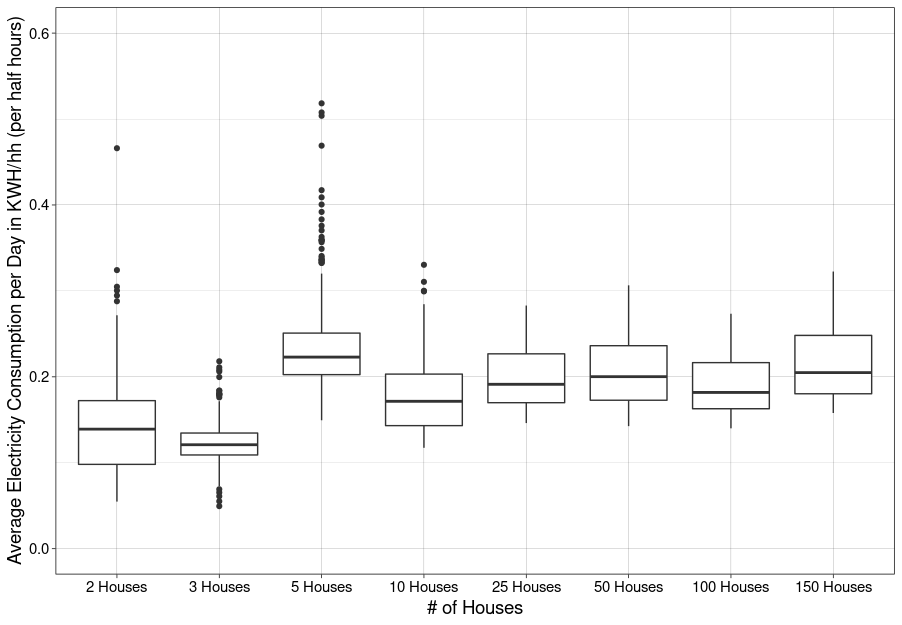
\includegraphics[width=0.85\textwidth]{images/boxplot_neu_neu.png}
\caption[Boxplots of the Average Base Load]{Boxplots of the Average Base Load}
\label{img:Box}
\end{figure}
\begin{figure}[!p]
\centering
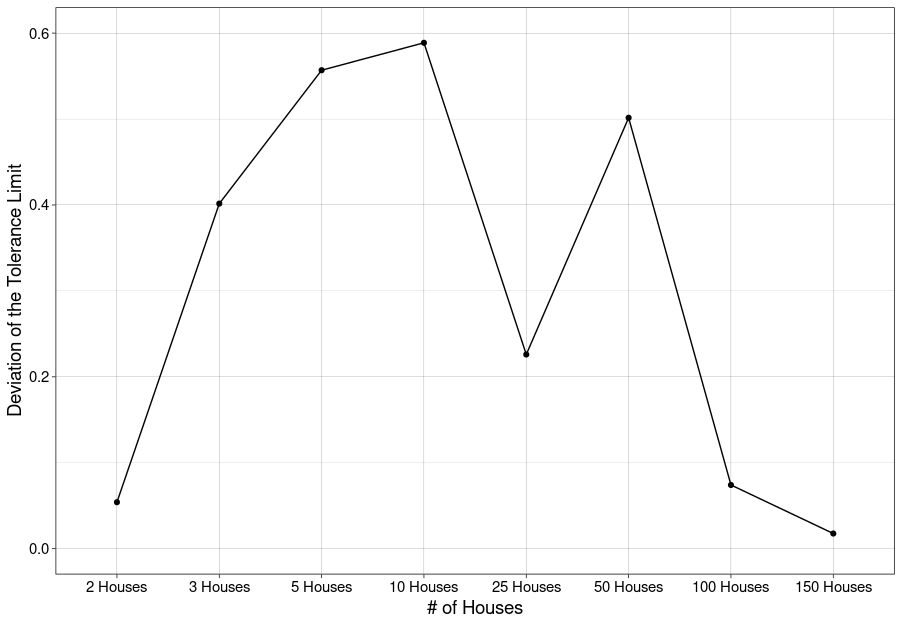
\includegraphics[width=0.85\textwidth]{images/Deviation_Houses.png}
\caption[Deviation of the Standard Variance]{Deviation of the Standard Variance}
\label{img:Deviation}
\end{figure}
\clearpage
}

%Nachschauen mit den ferien im april bei 2 häusern
%durchschnittliche Mittelwert(von boxplots)
%ergebnisse der abweichung
%versuche wurden 2 mal wiederholt.
\afterpage{%
\begin{figure}[!p]
\centering
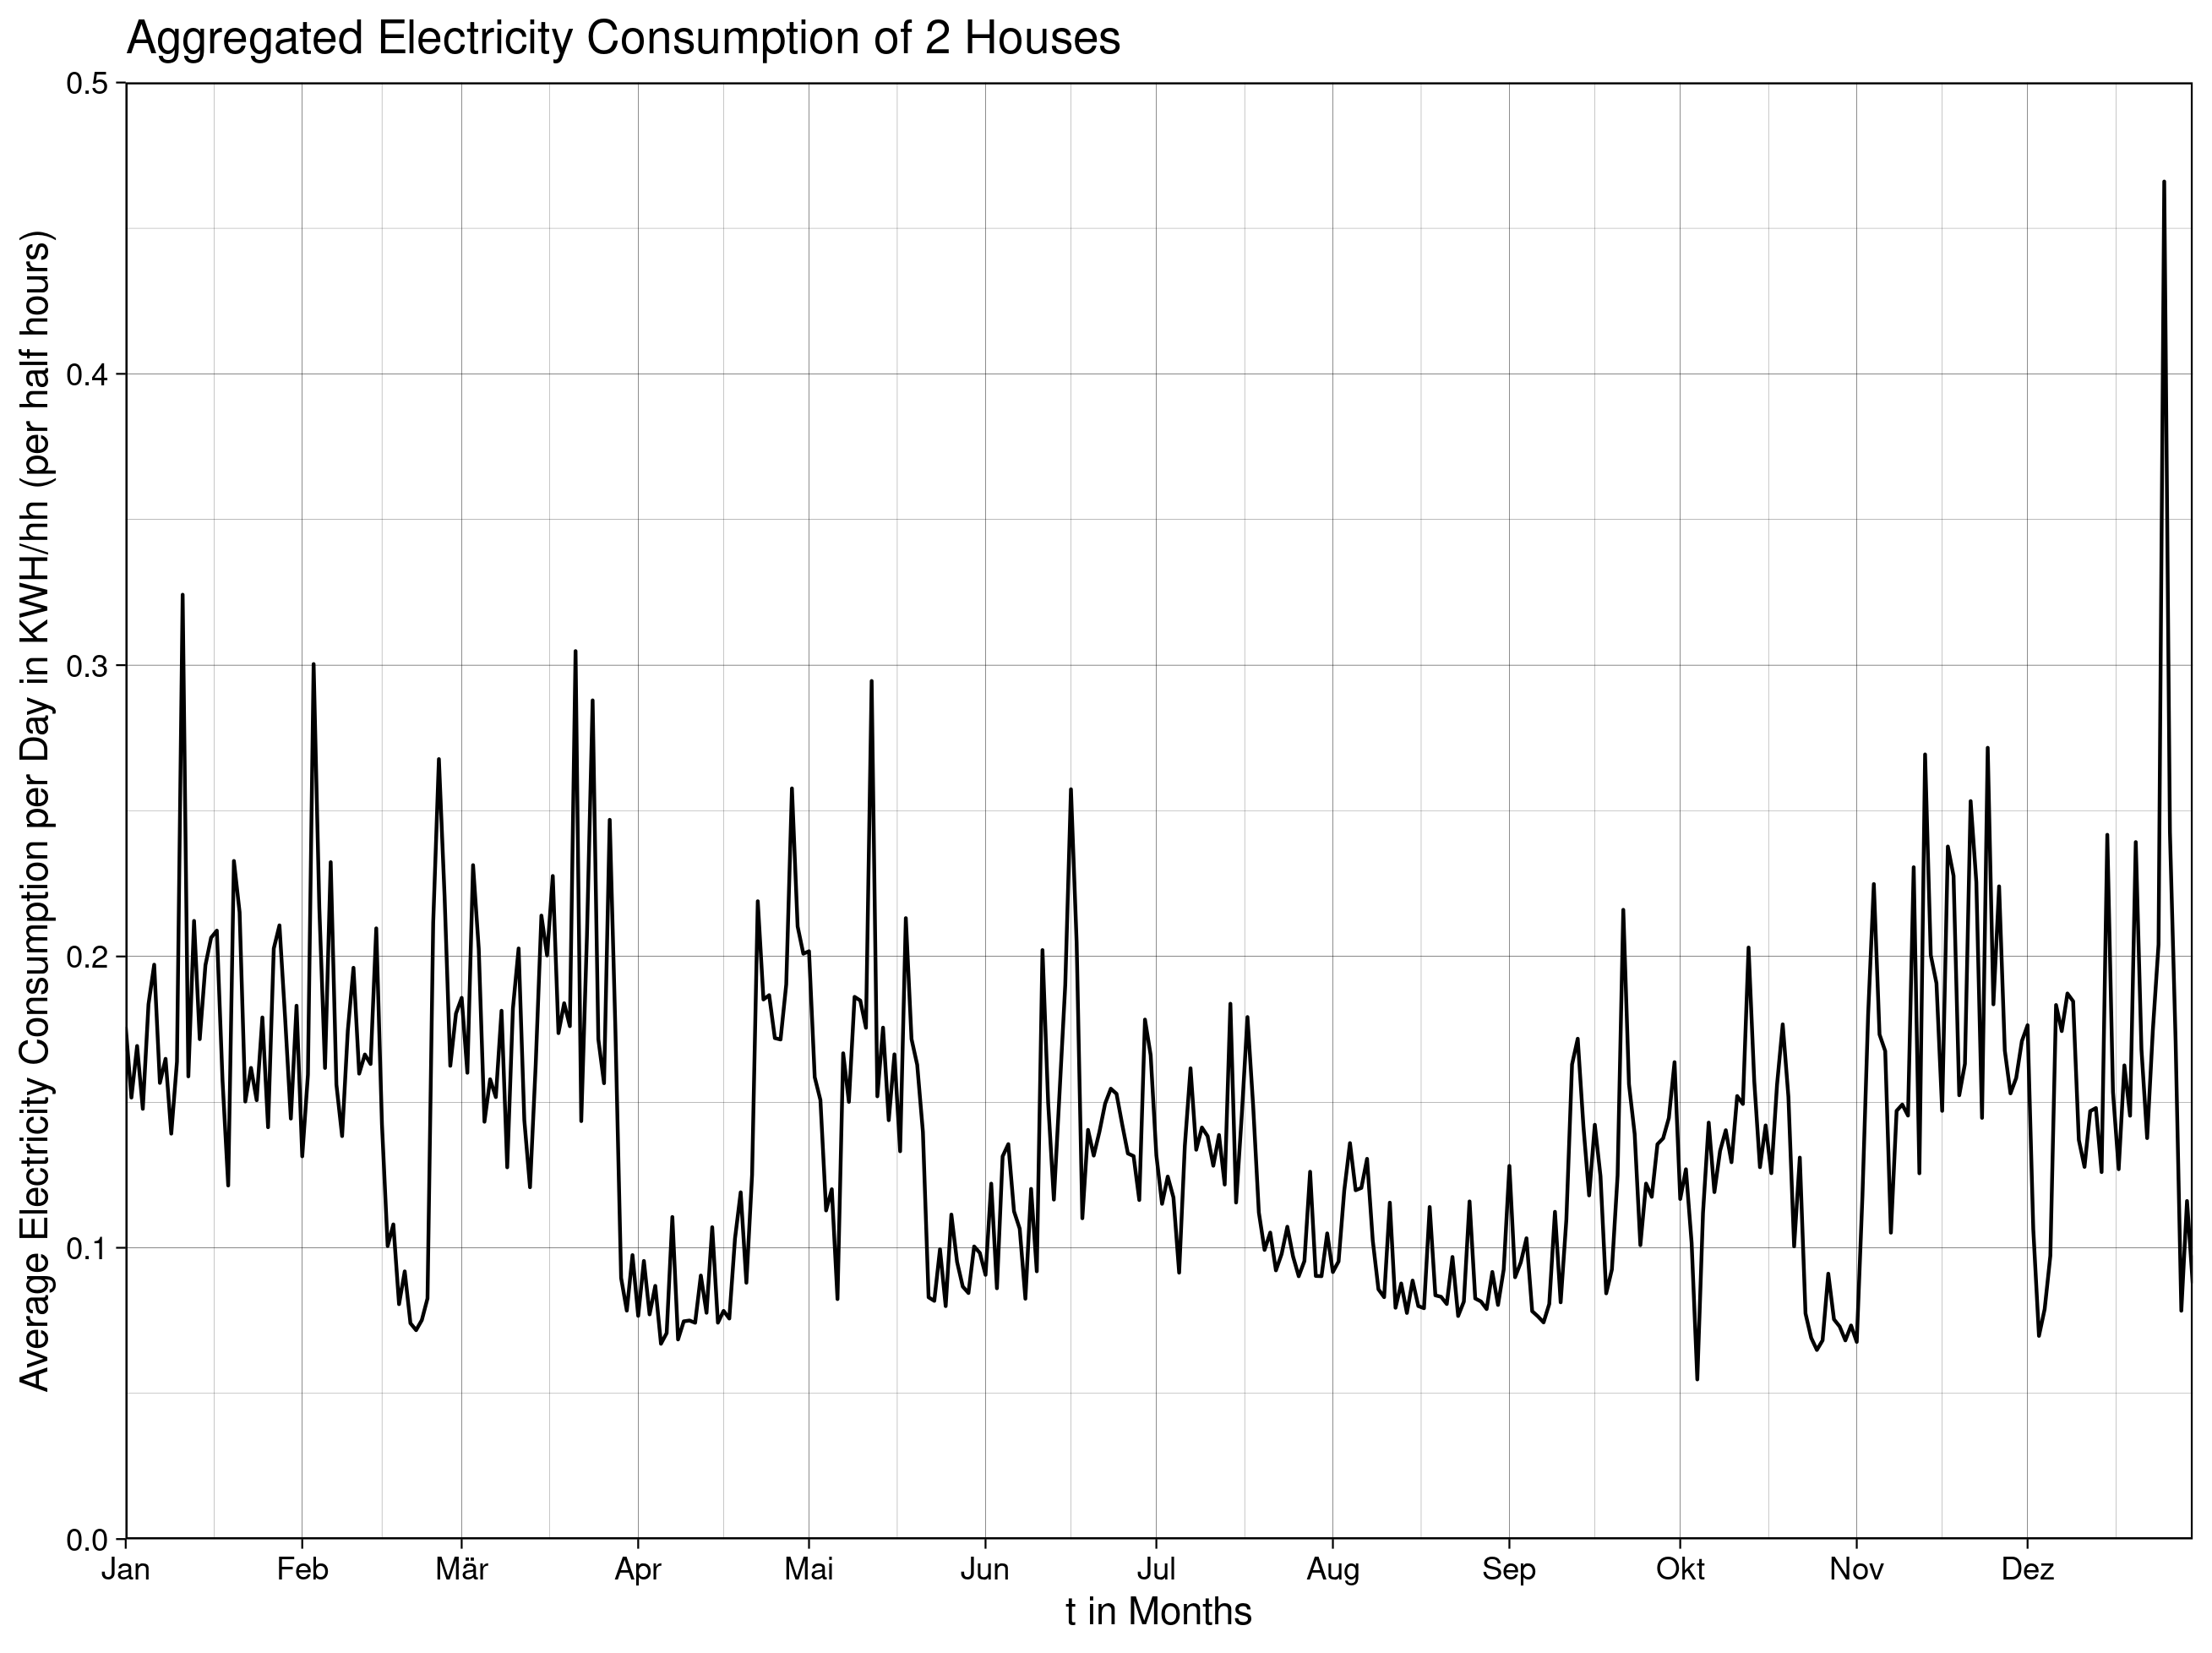
\includegraphics[width=0.85\textwidth]{images/Aggregated Electricity Consumption of 2 Houses.png}
\caption[Aggregated Electricity Consumption of 2 Houses]{}
\label{img:2_Houses}
\end{figure}
\begin{figure}[!p]
\centering
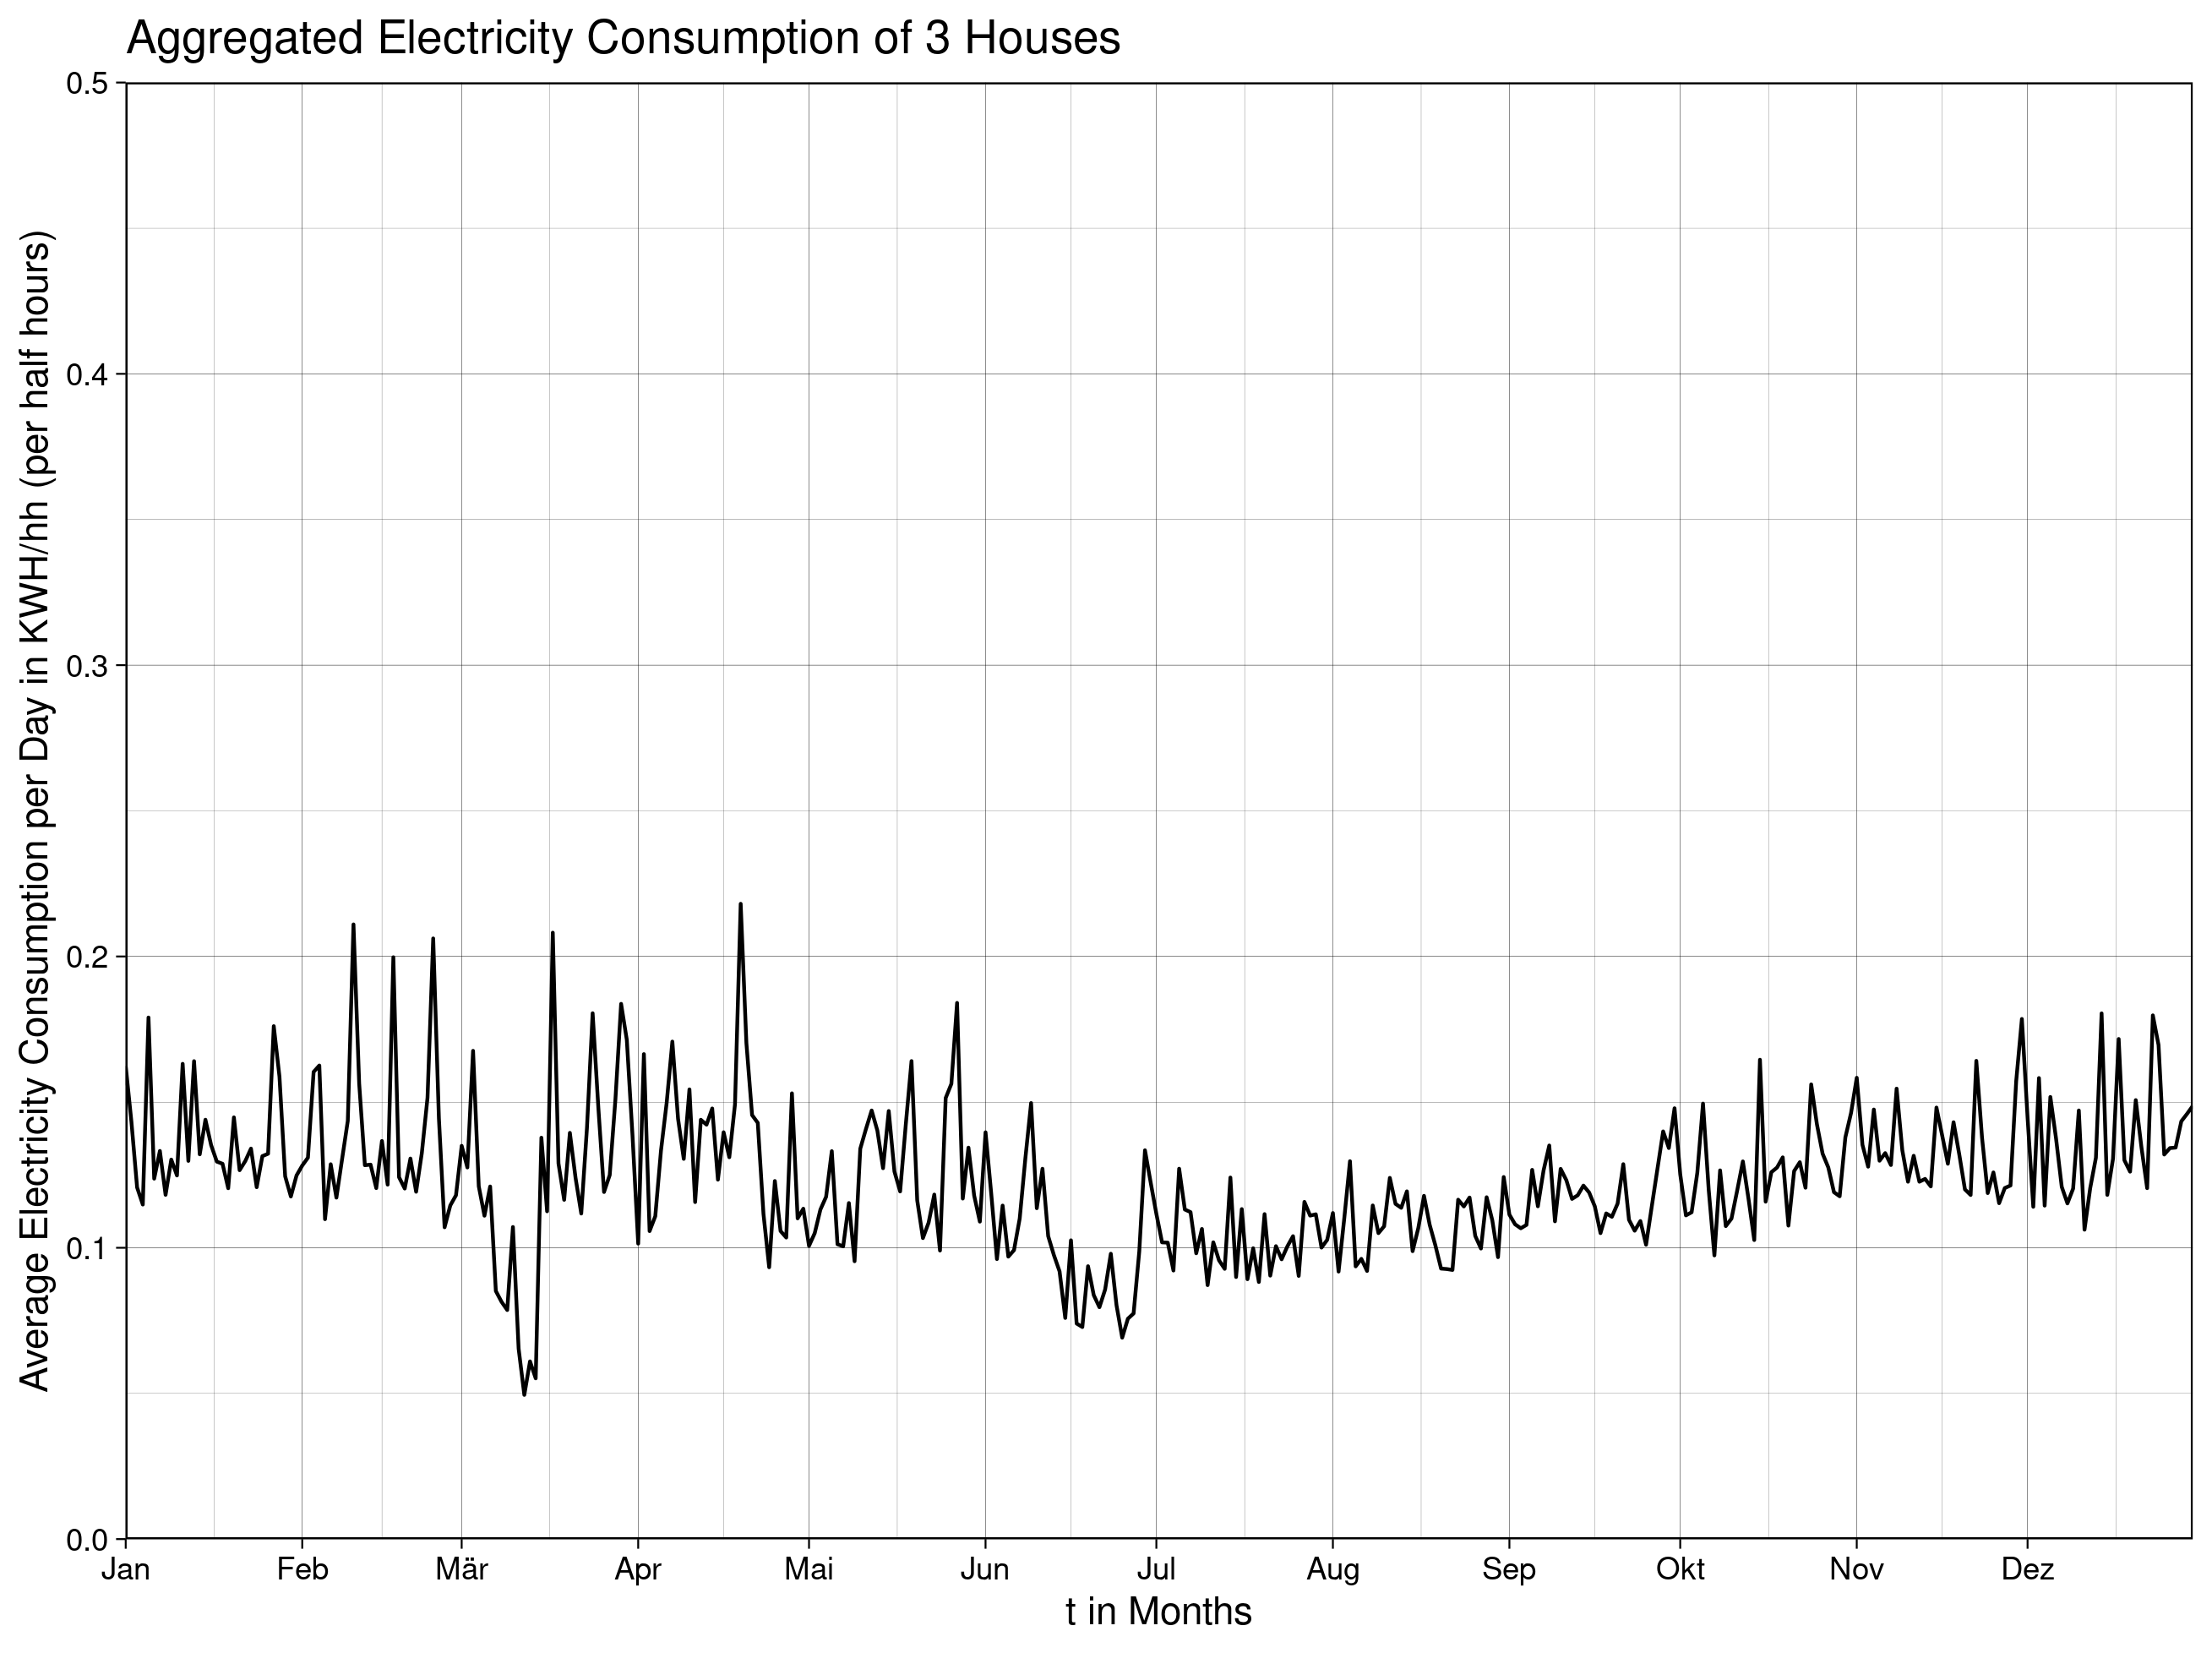
\includegraphics[width=0.85\textwidth]{images/Aggregated Electricity Consumption of 3 Houses.png}
\caption[Aggregated Electricity Consumption of 3 Houses]{}
\label{img:3_Houses}
\end{figure}
\clearpage
}
\afterpage{%
\begin{figure}[!p]
\centering
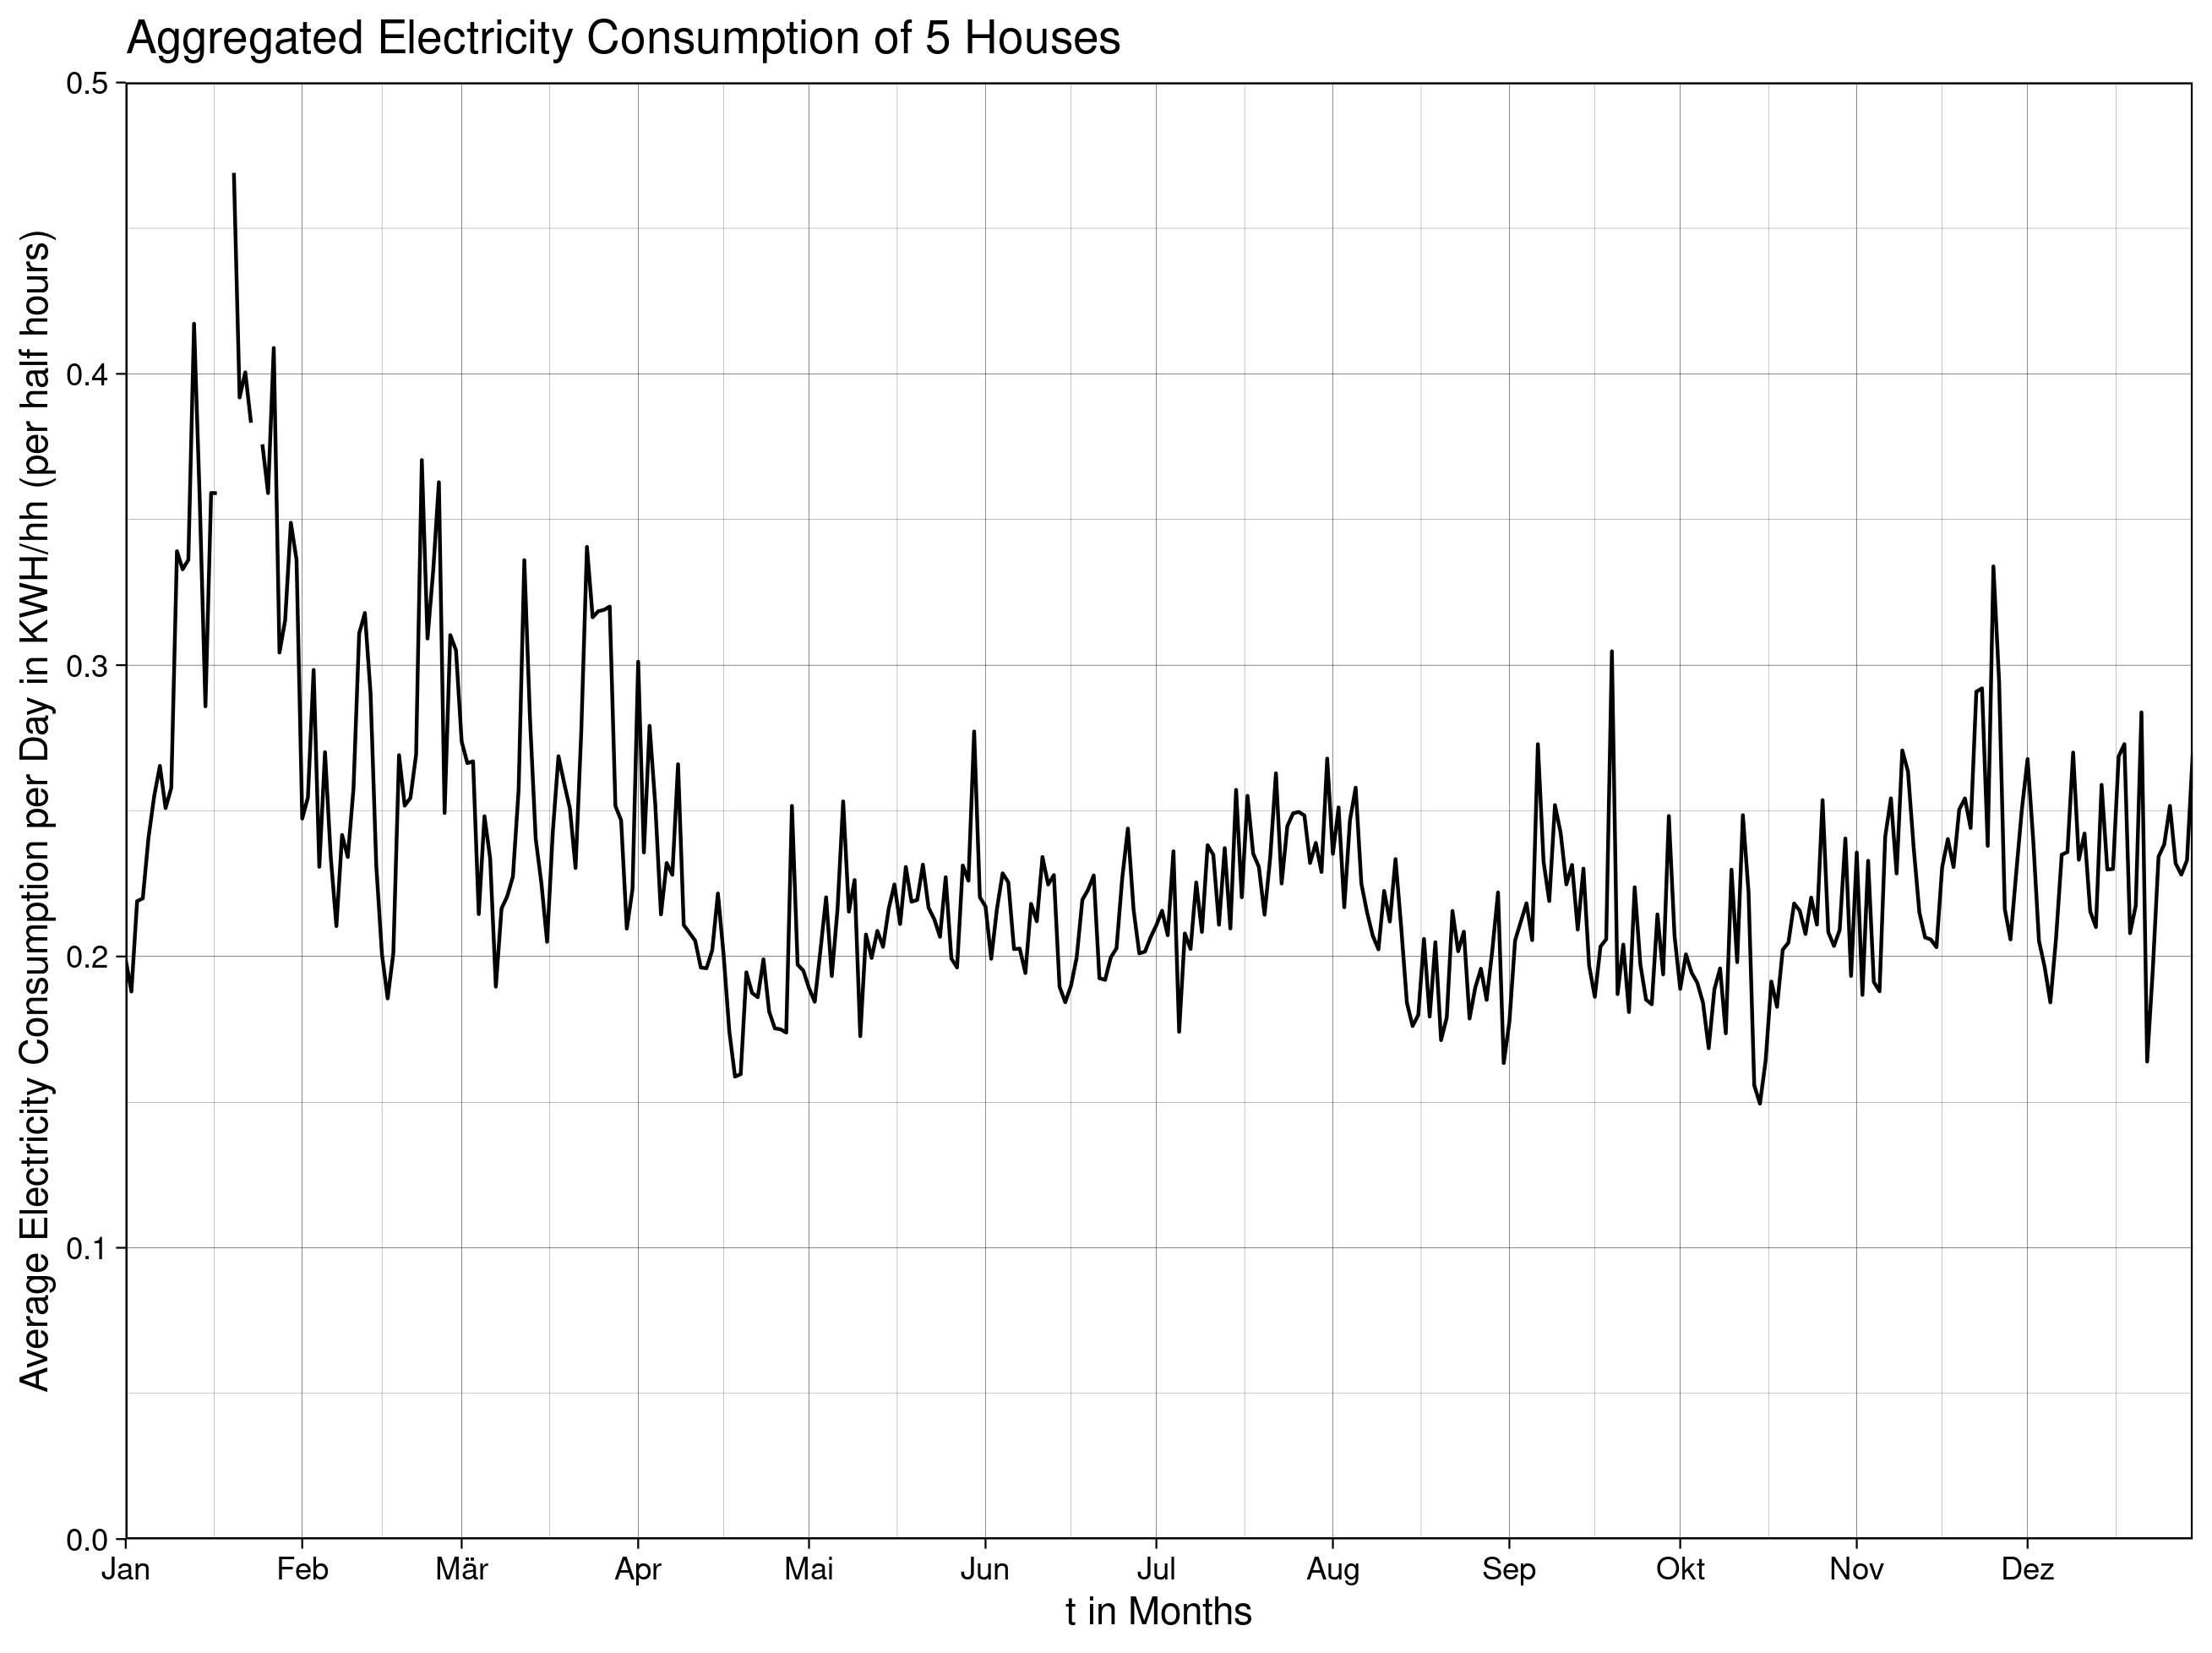
\includegraphics[width=0.85\textwidth]{images/Aggregated Electricity Consumption of 5 Houses.png}
\caption[Aggregated Electricity Consumption of 5 Houses]{}
\label{img:5_Houses}
\end{figure}
\begin{figure}[!p]
\centering
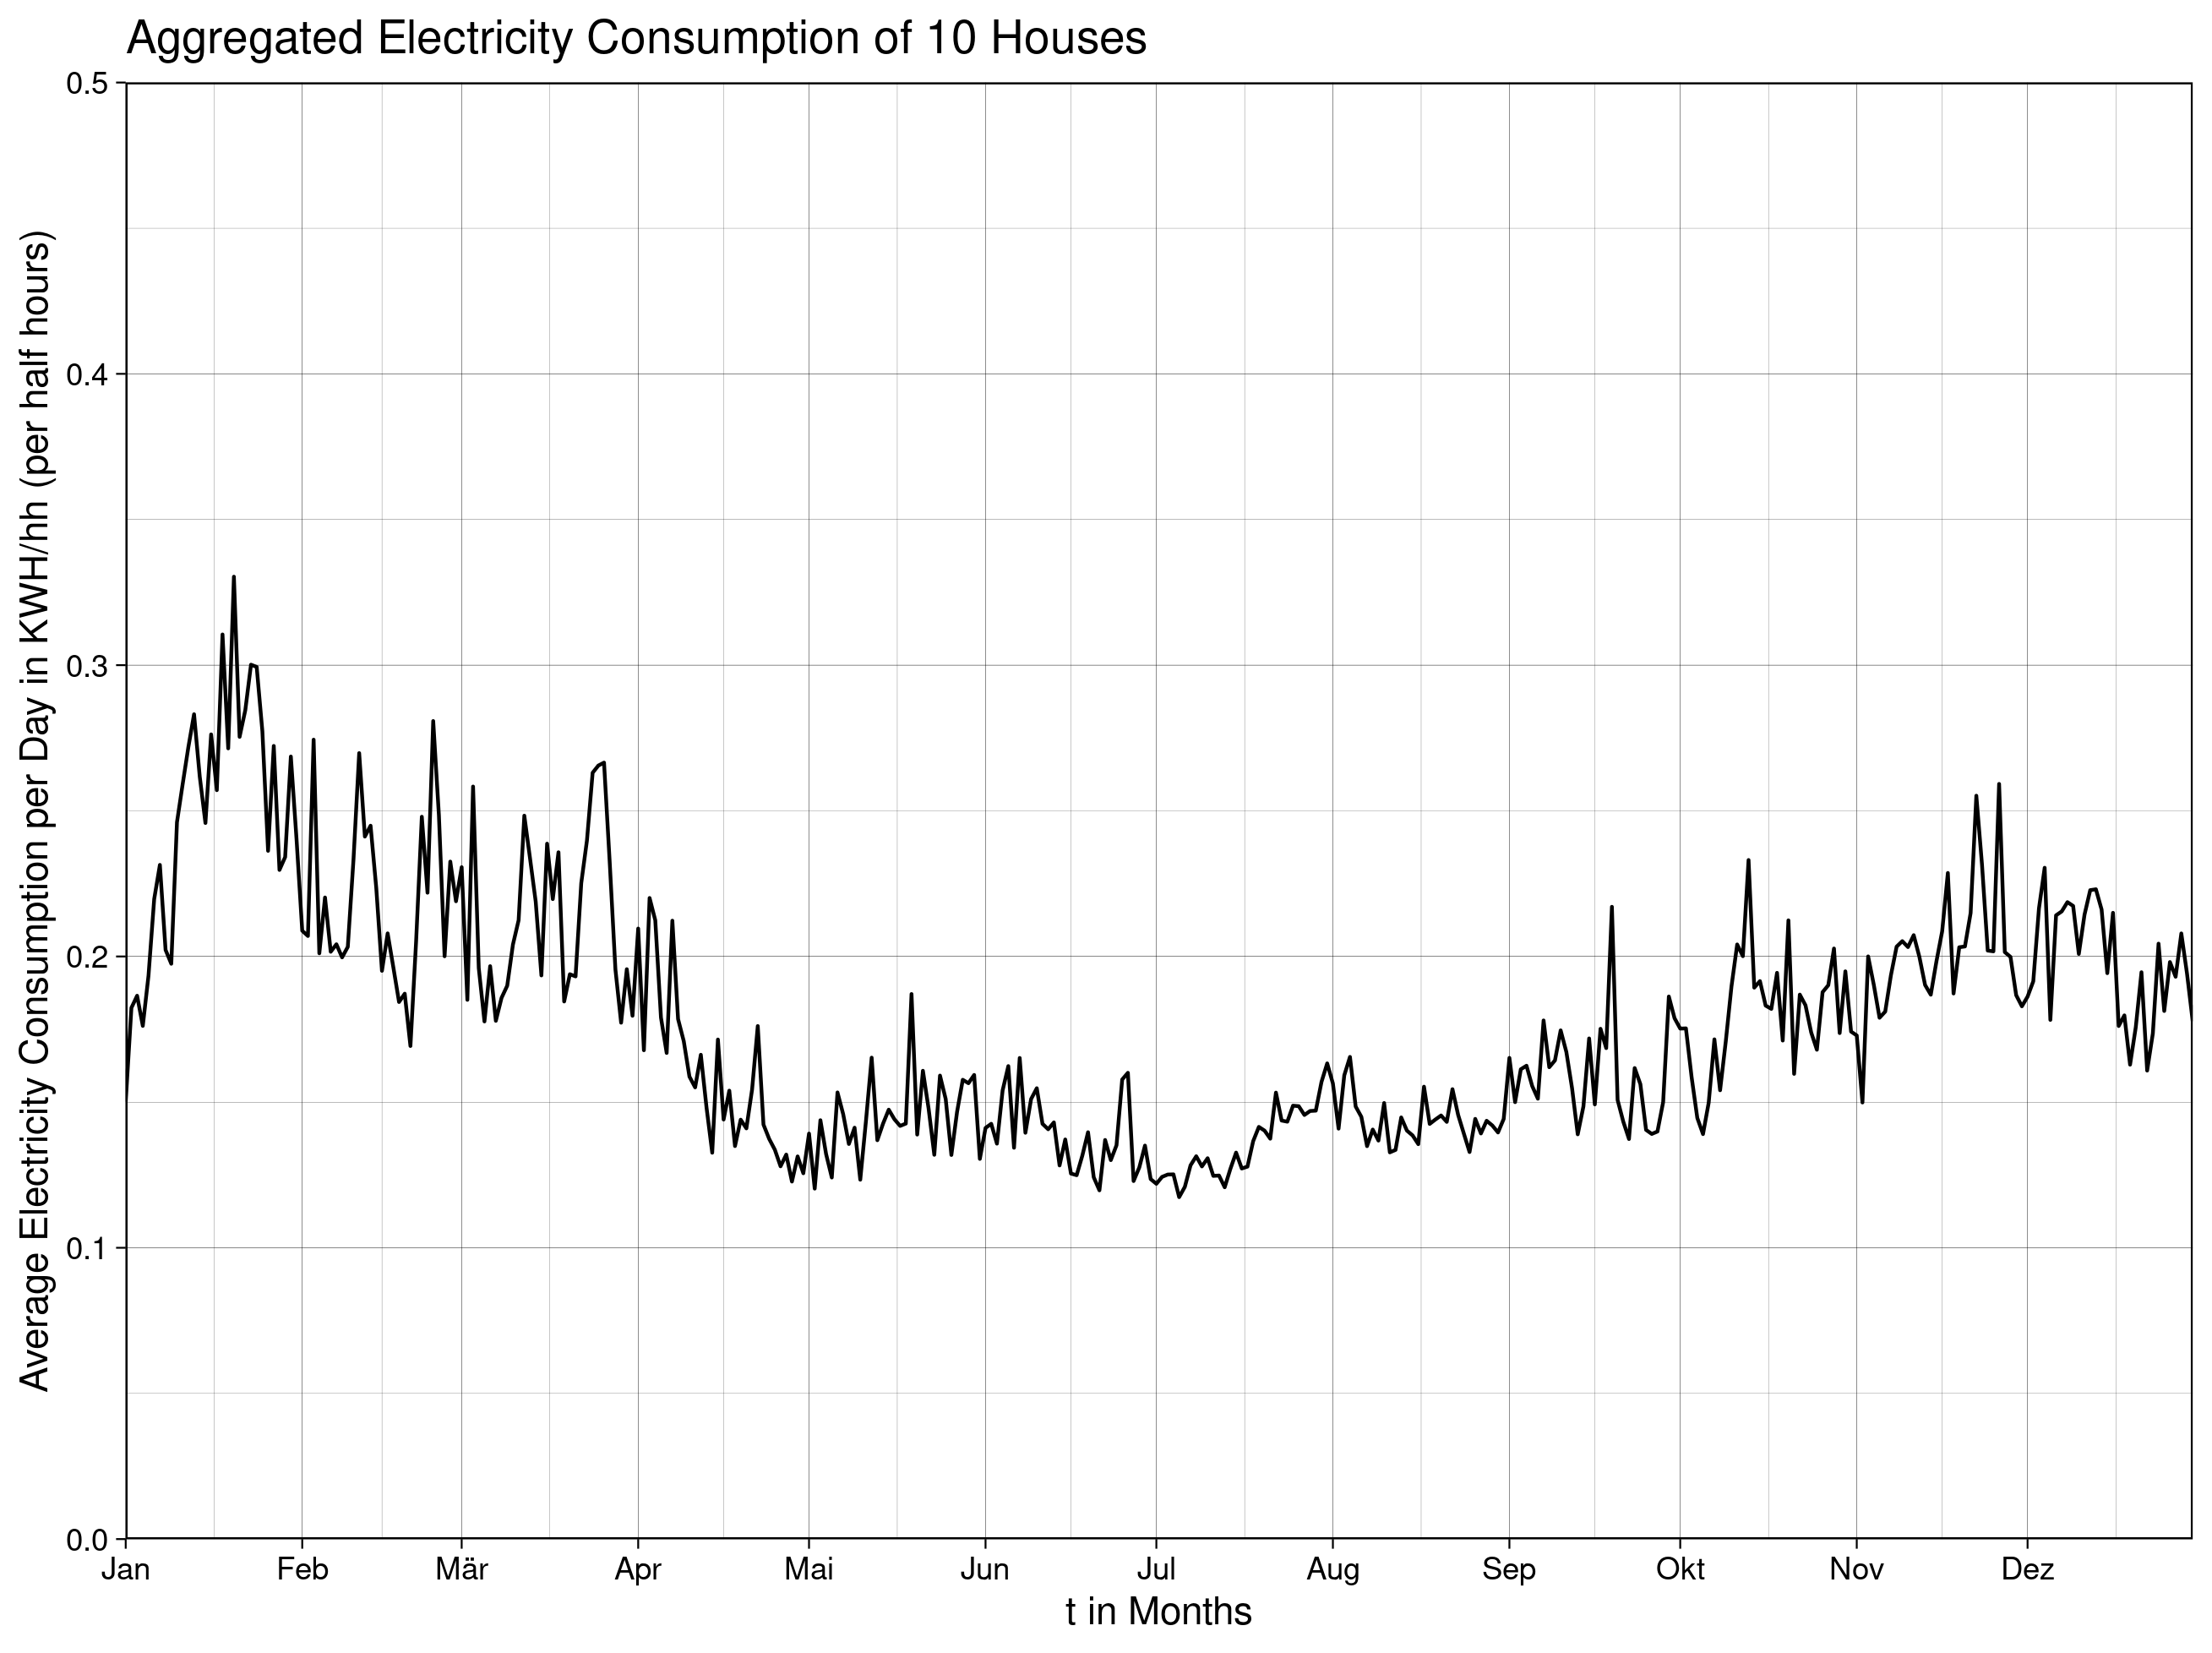
\includegraphics[width=0.85\textwidth]{images/Aggregated Electricity Consumption of 10 Houses.png}
\caption[Aggregated Electricity Consumption of 10 Houses]{}
\label{img:10_Houses}
\end{figure}
\clearpage
}
\afterpage{%
\begin{figure}[!p]
\centering
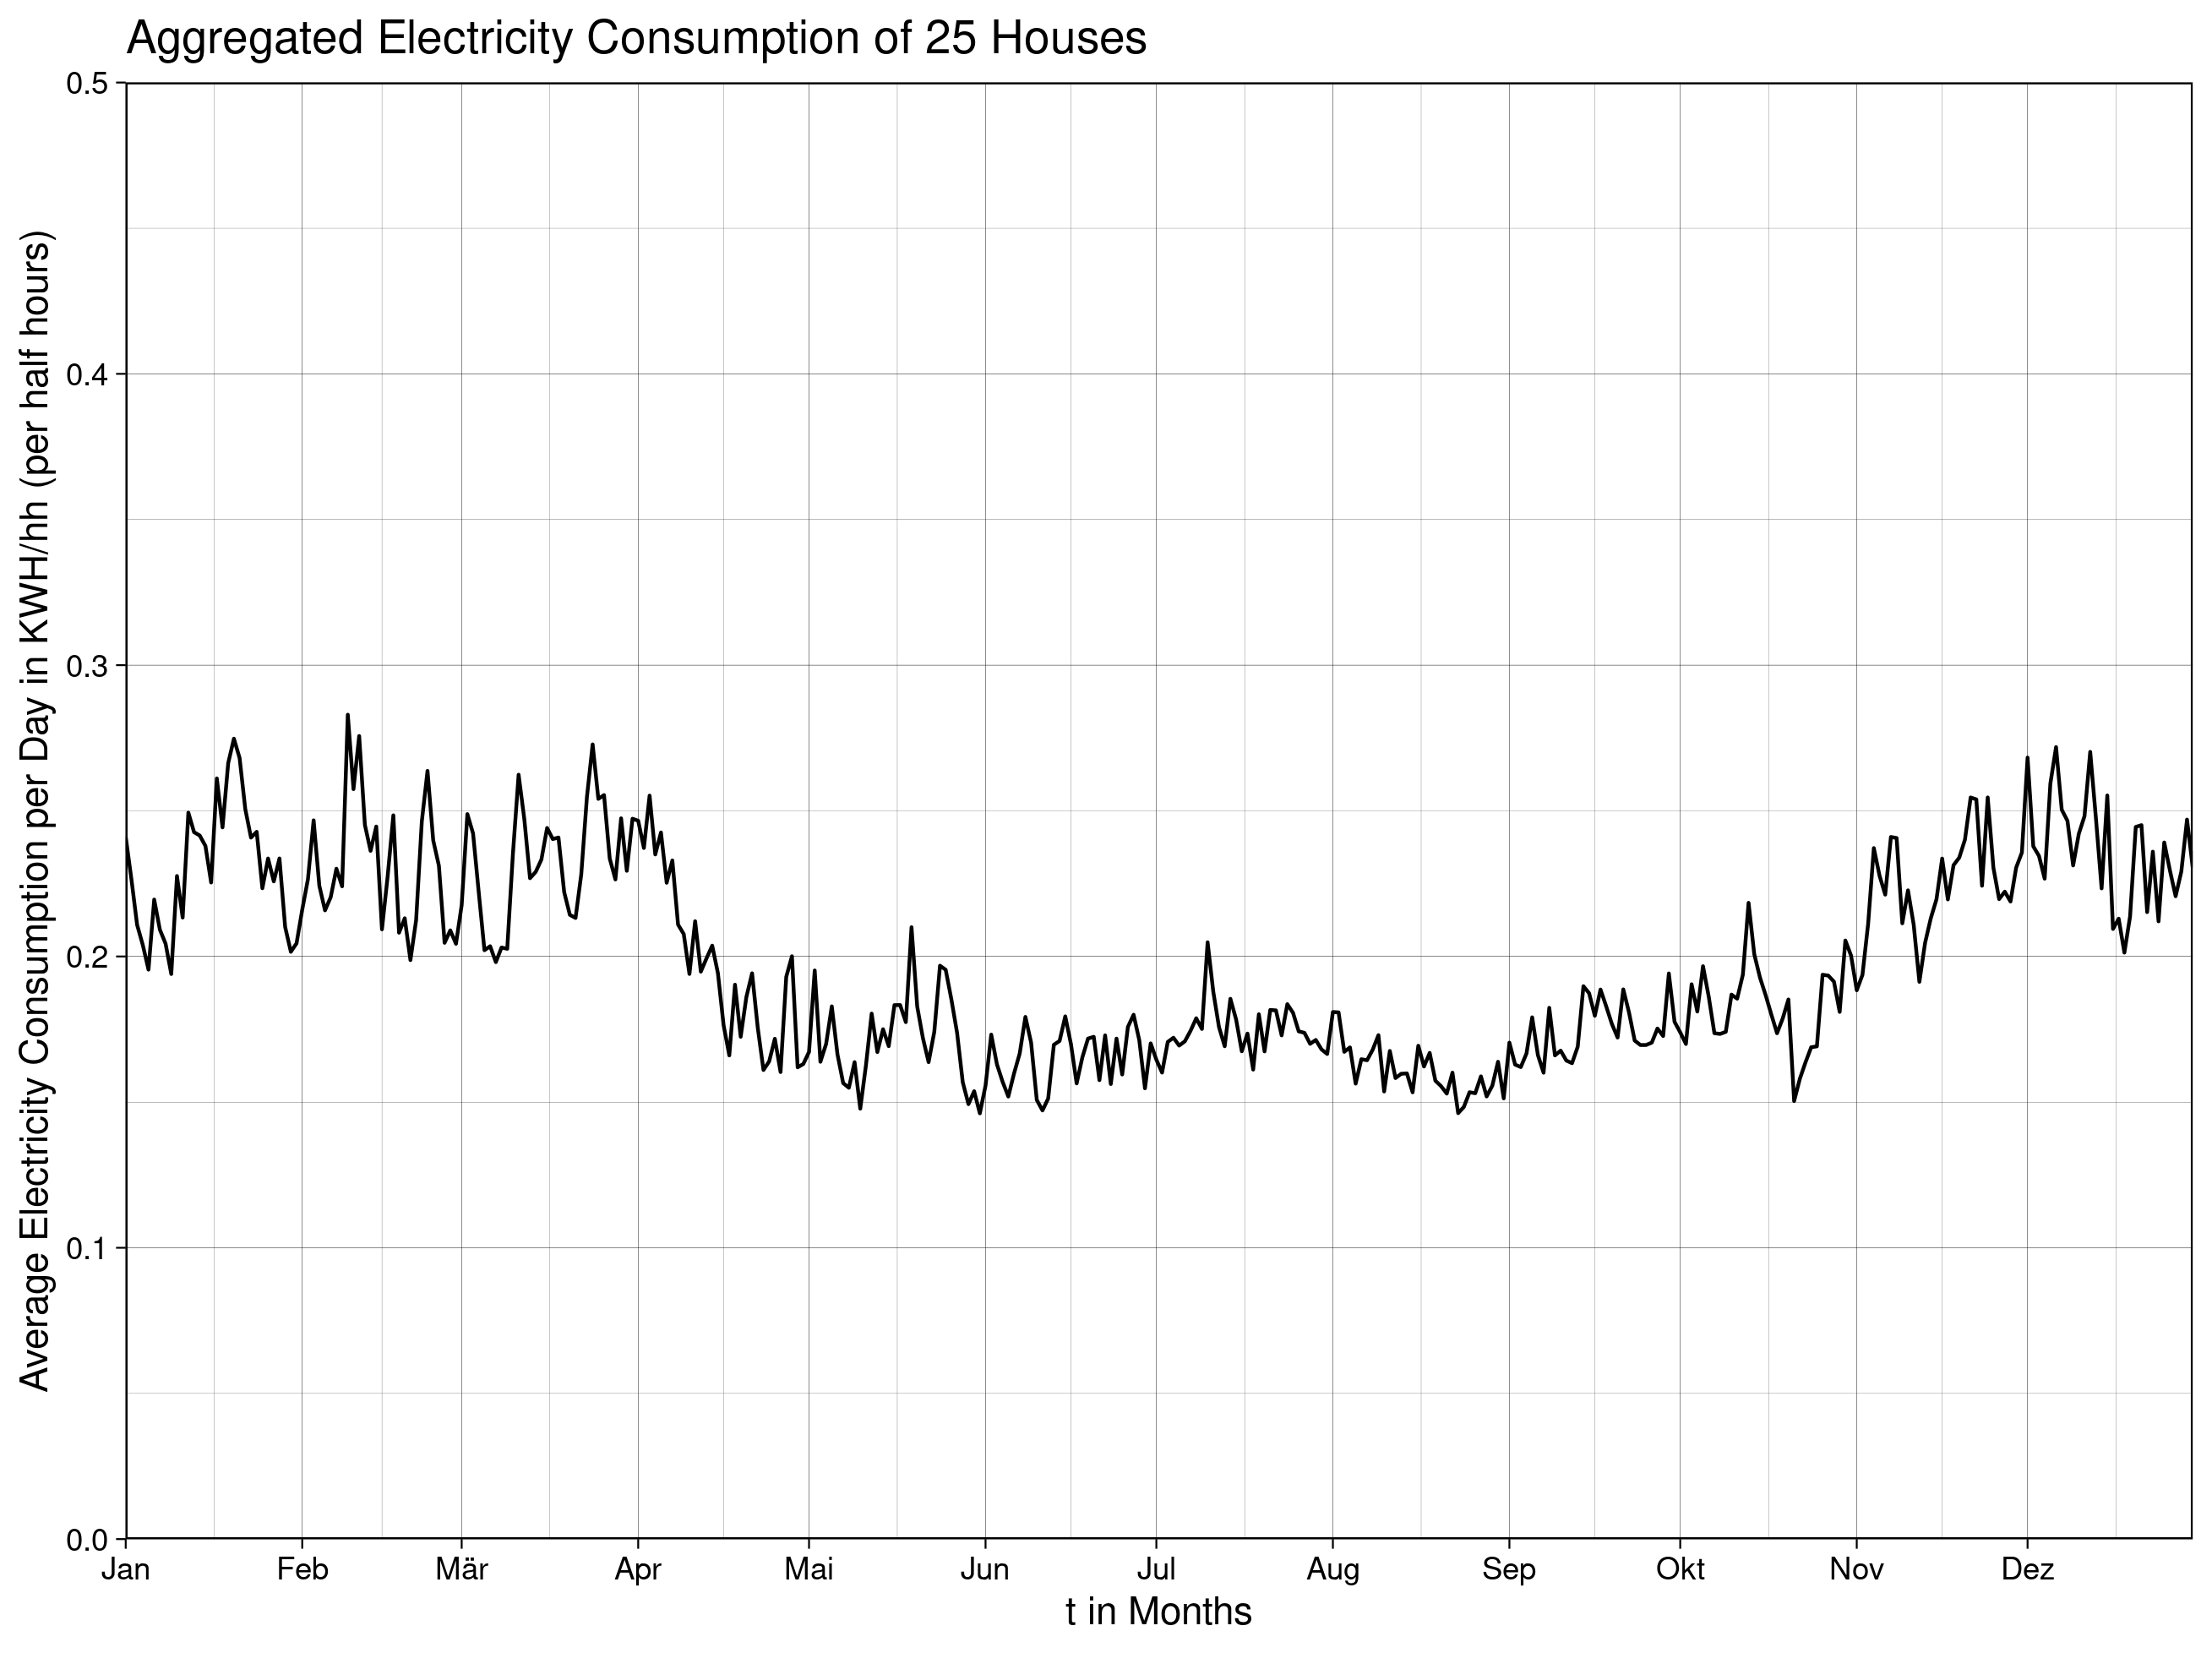
\includegraphics[width=0.85\textwidth]{images/Aggregated Electricity Consumption of 25 Houses.png}
\caption[Aggregated Electricity Consumption of 25 Houses]{}
\label{img:25_Houses}
\end{figure}
\begin{figure}[!p]
\centering
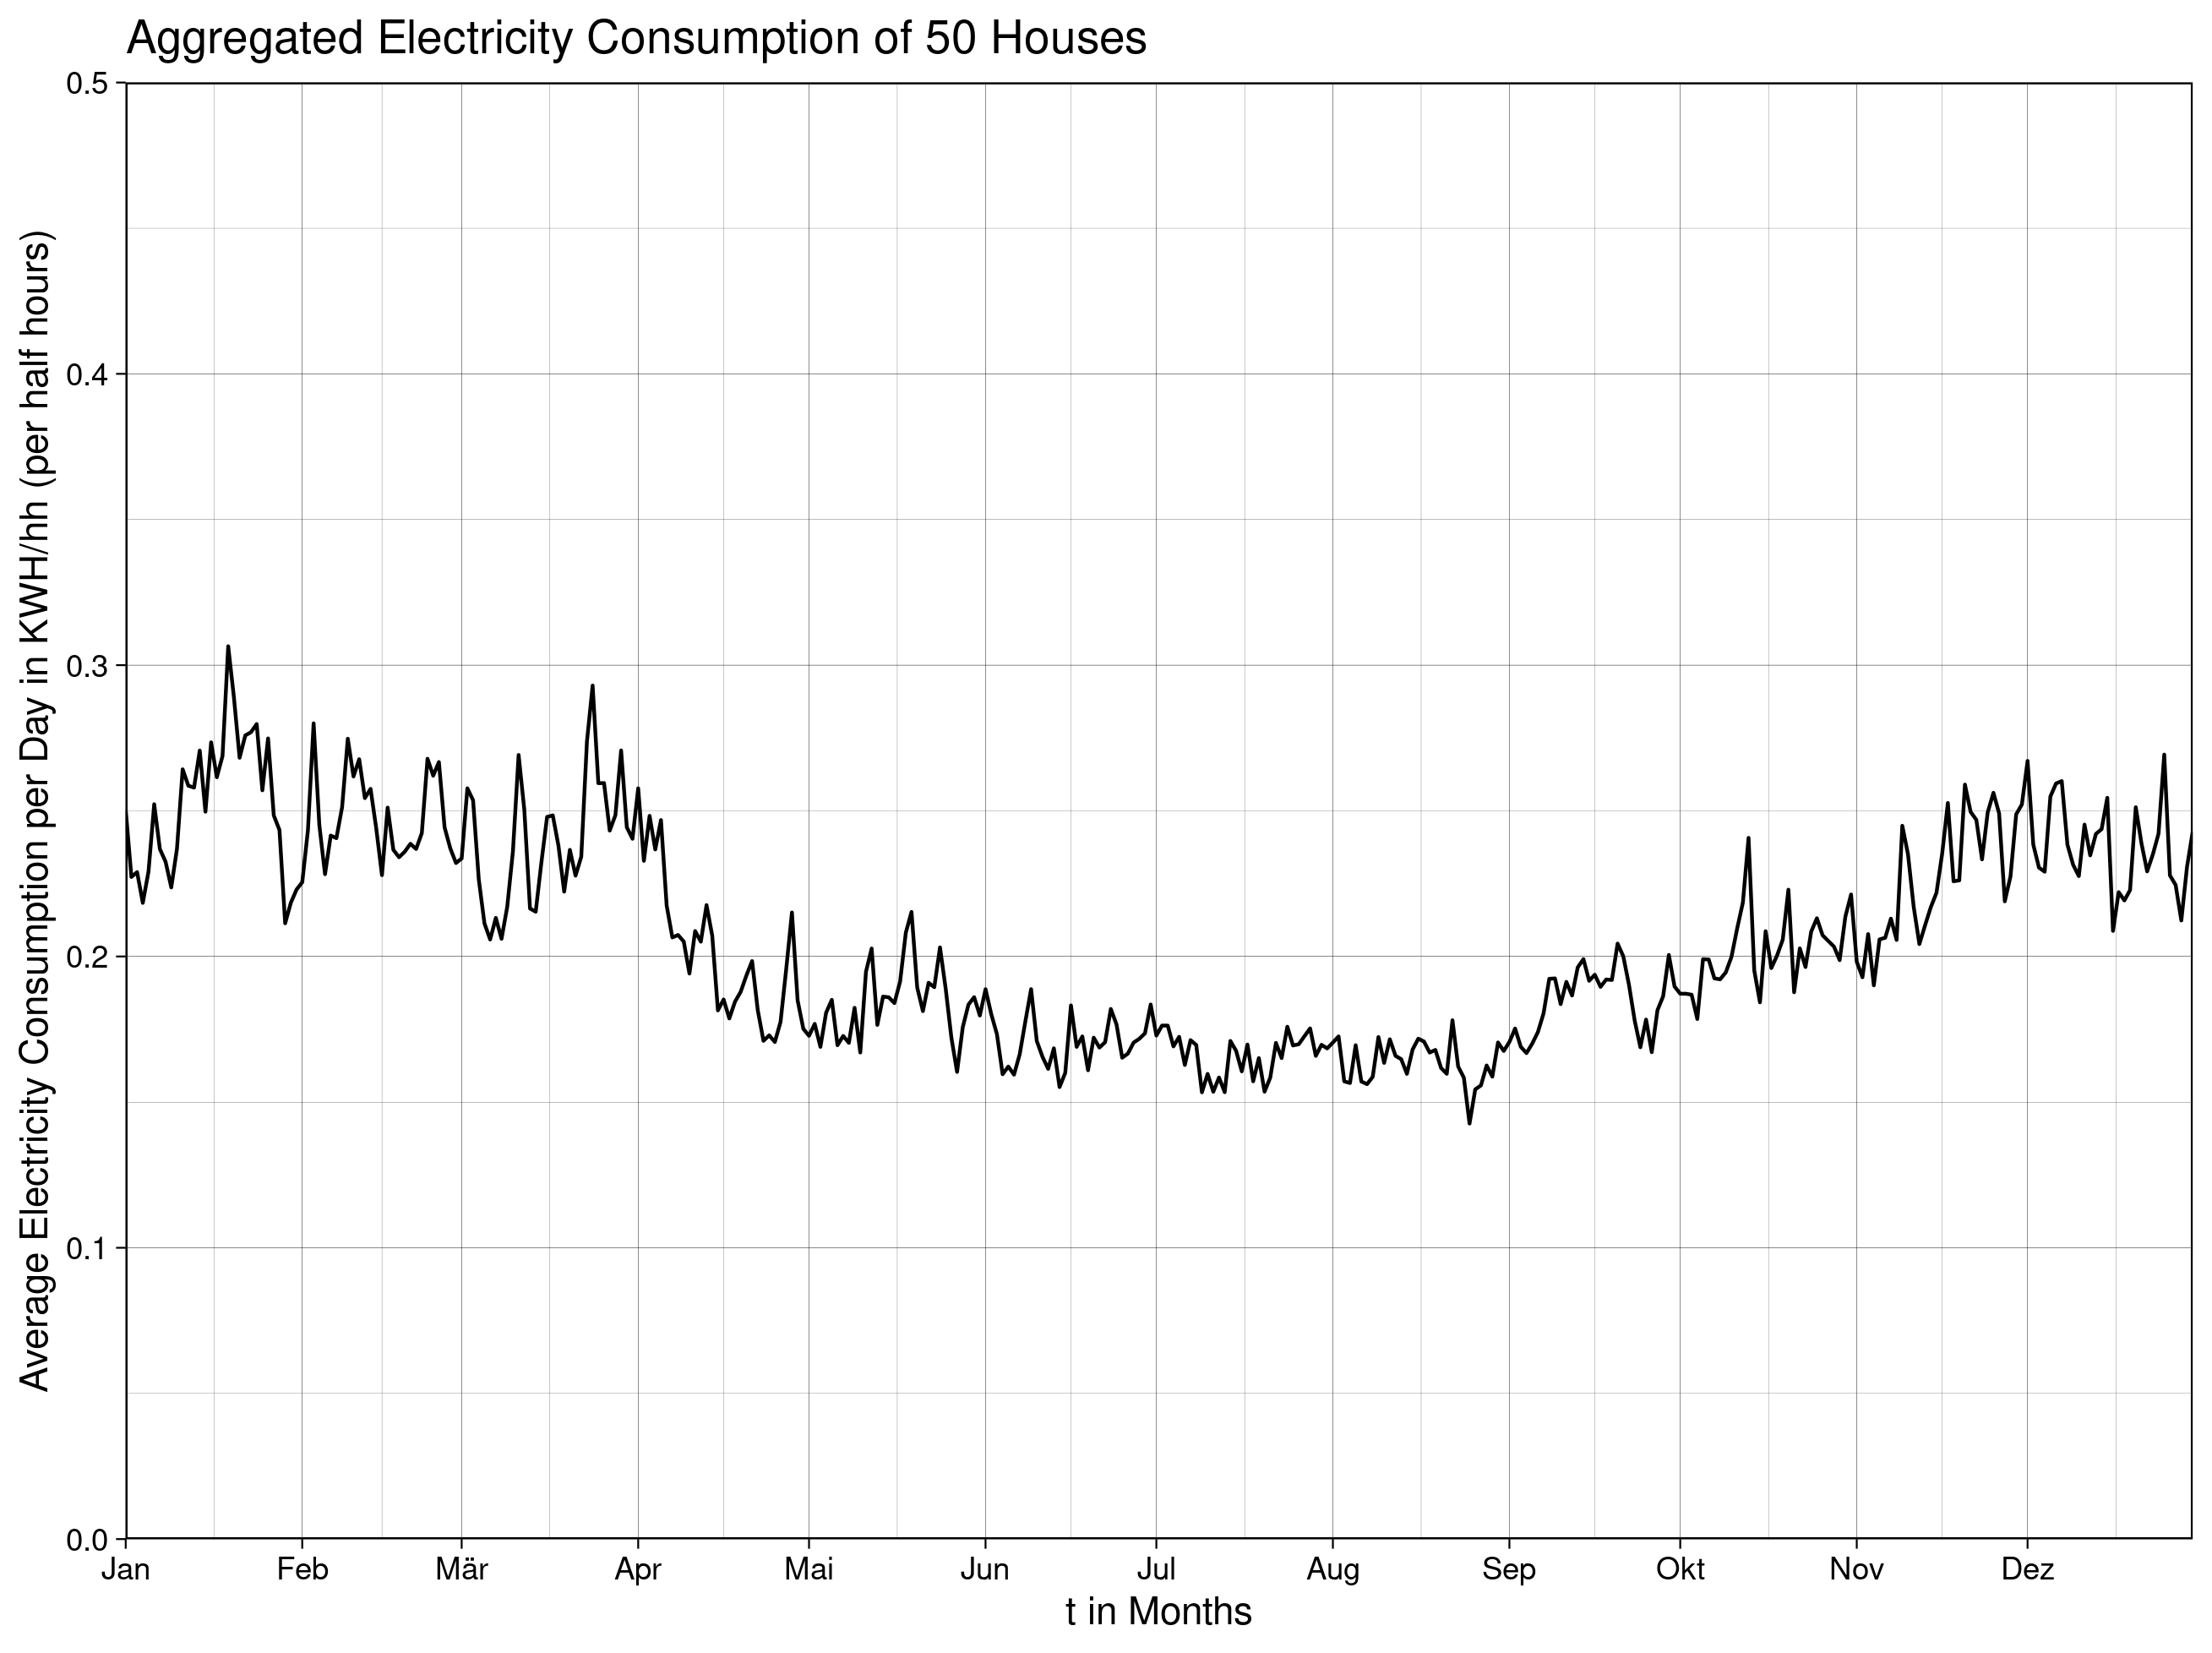
\includegraphics[width=0.85\textwidth]{images/Aggregated Electricity Consumption of 50 Houses.png}
\caption[Aggregated Electricity Consumption of 50 Houses]{}
\label{img:50_Houses}
\end{figure}
\clearpage
}
\afterpage{%
\begin{figure}[!p]
\centering
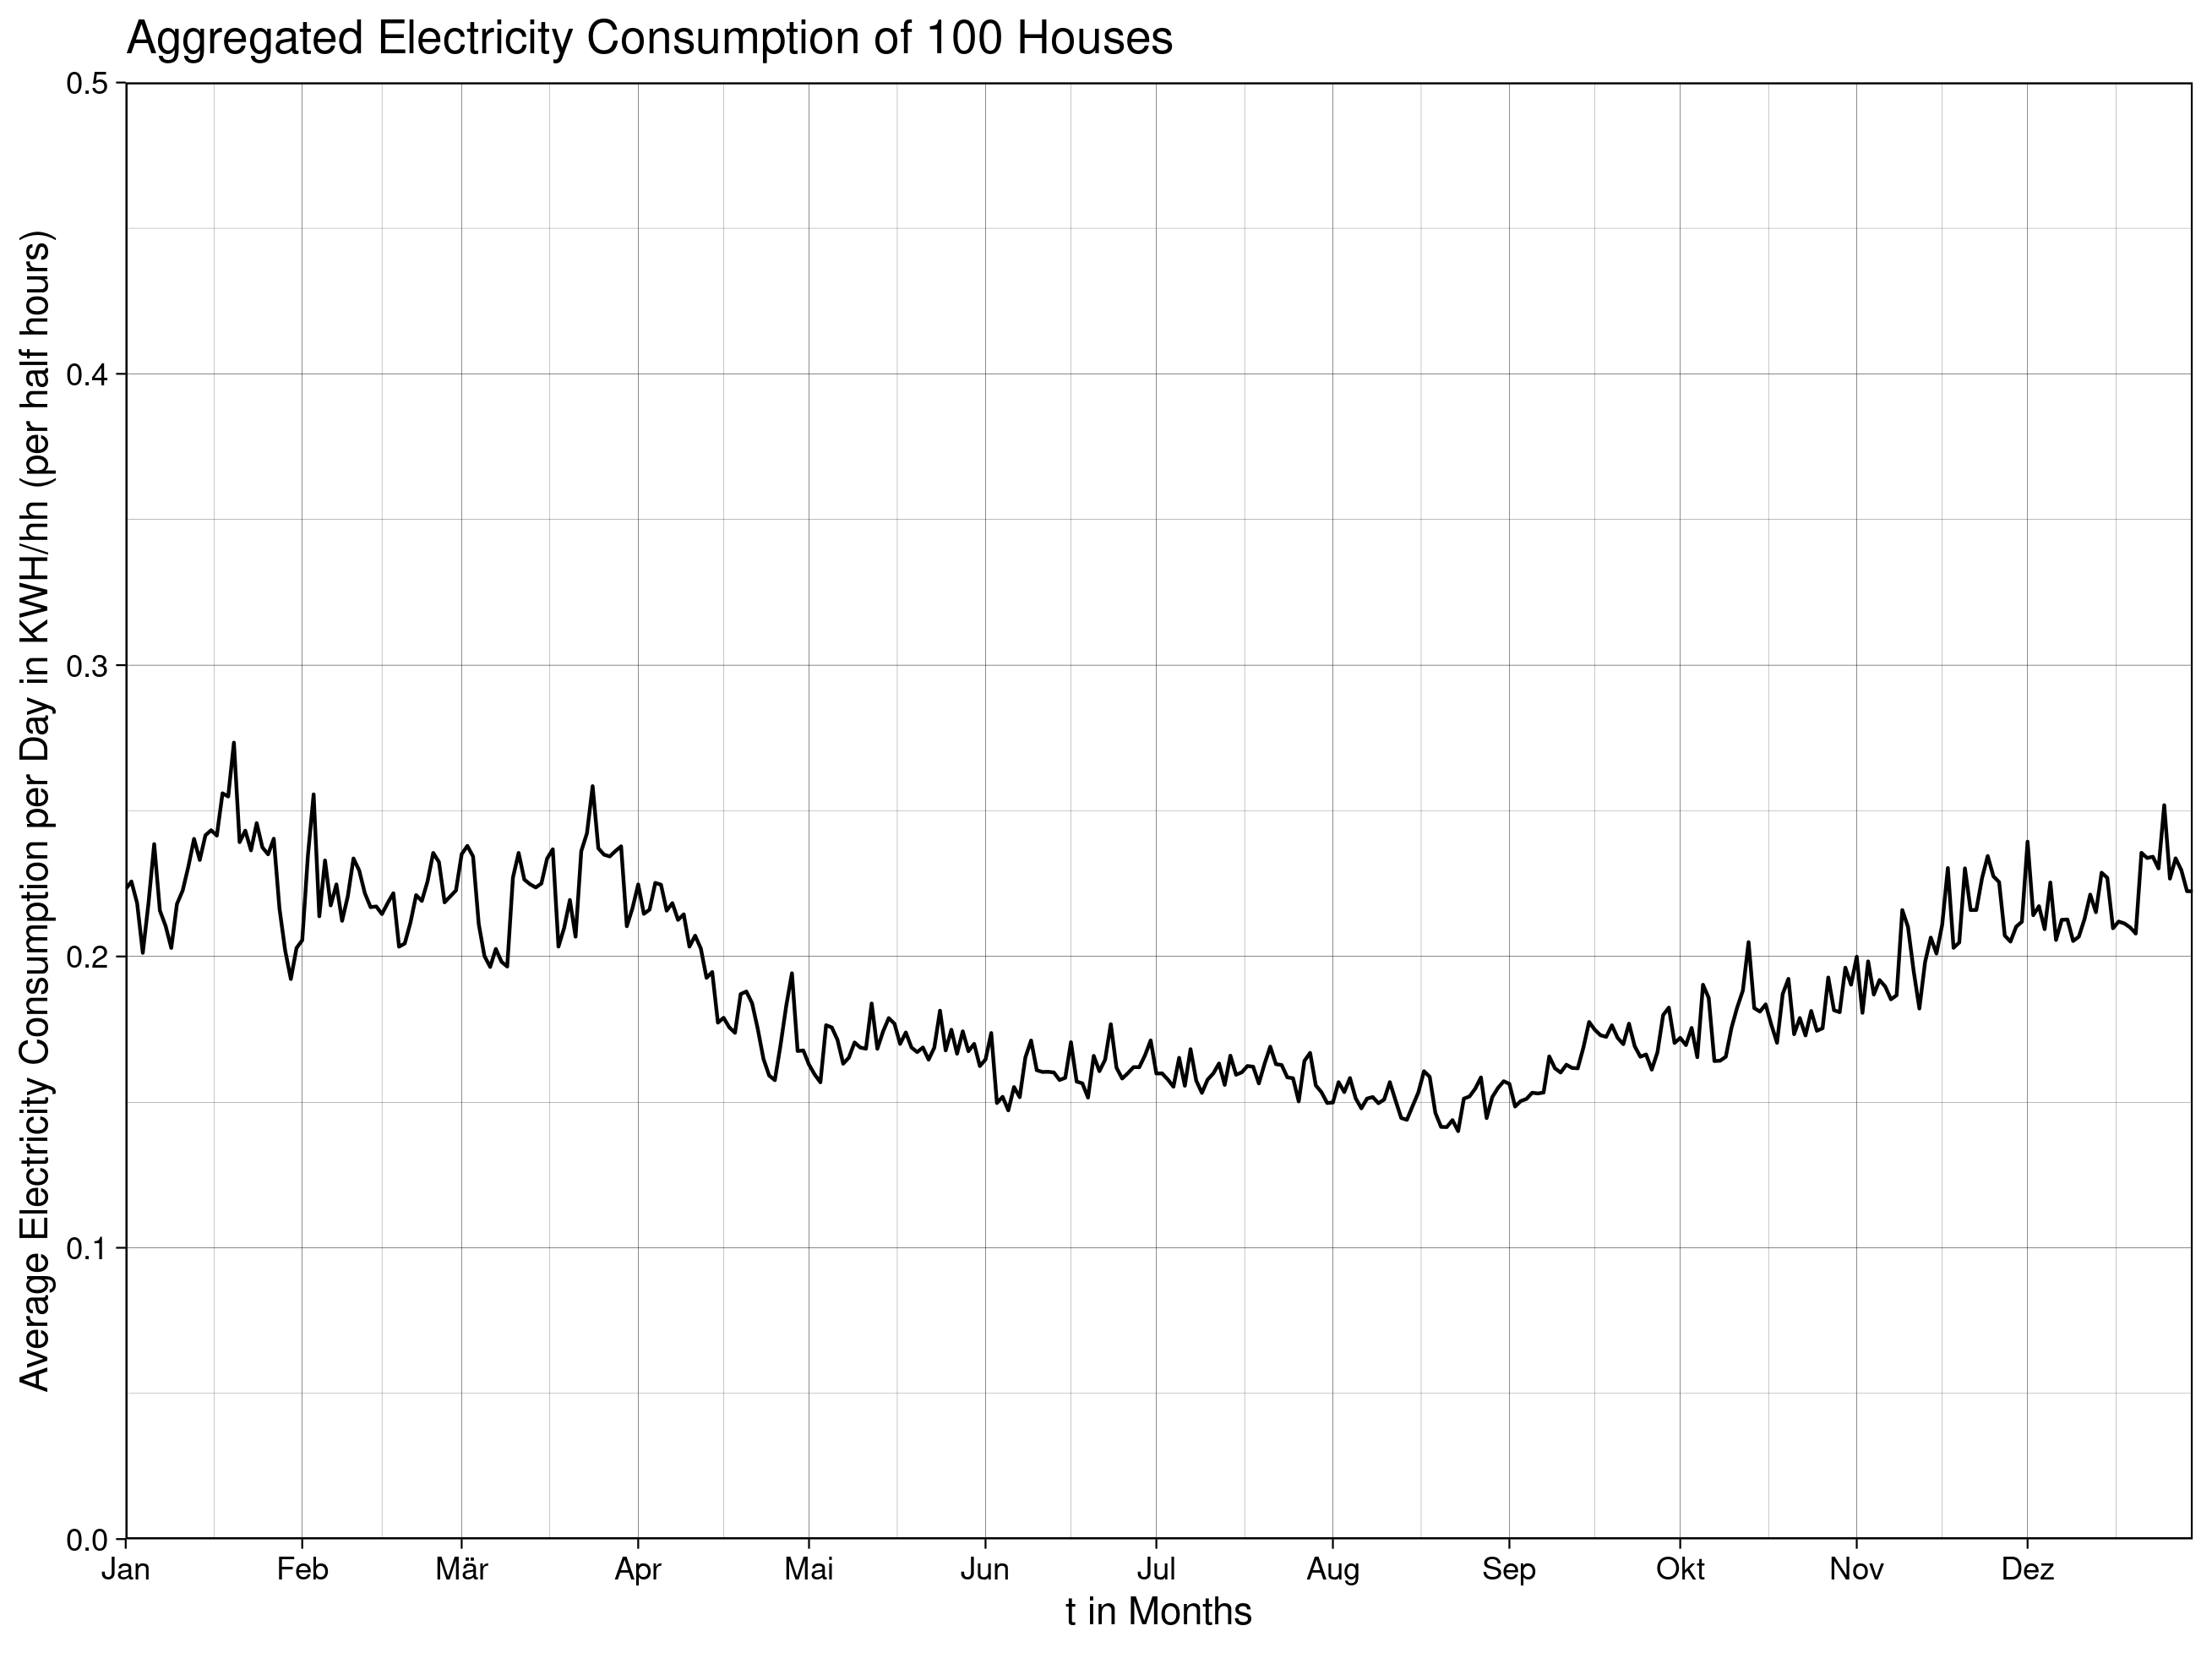
\includegraphics[width=0.85\textwidth]{images/Aggregated Electricity Consumption of 100 Houses.png}
\caption[Aggregated Electricity Consumption of 100 Houses]{}
\label{img:100_Houses}
\end{figure}
\begin{figure}[!p]
\centering
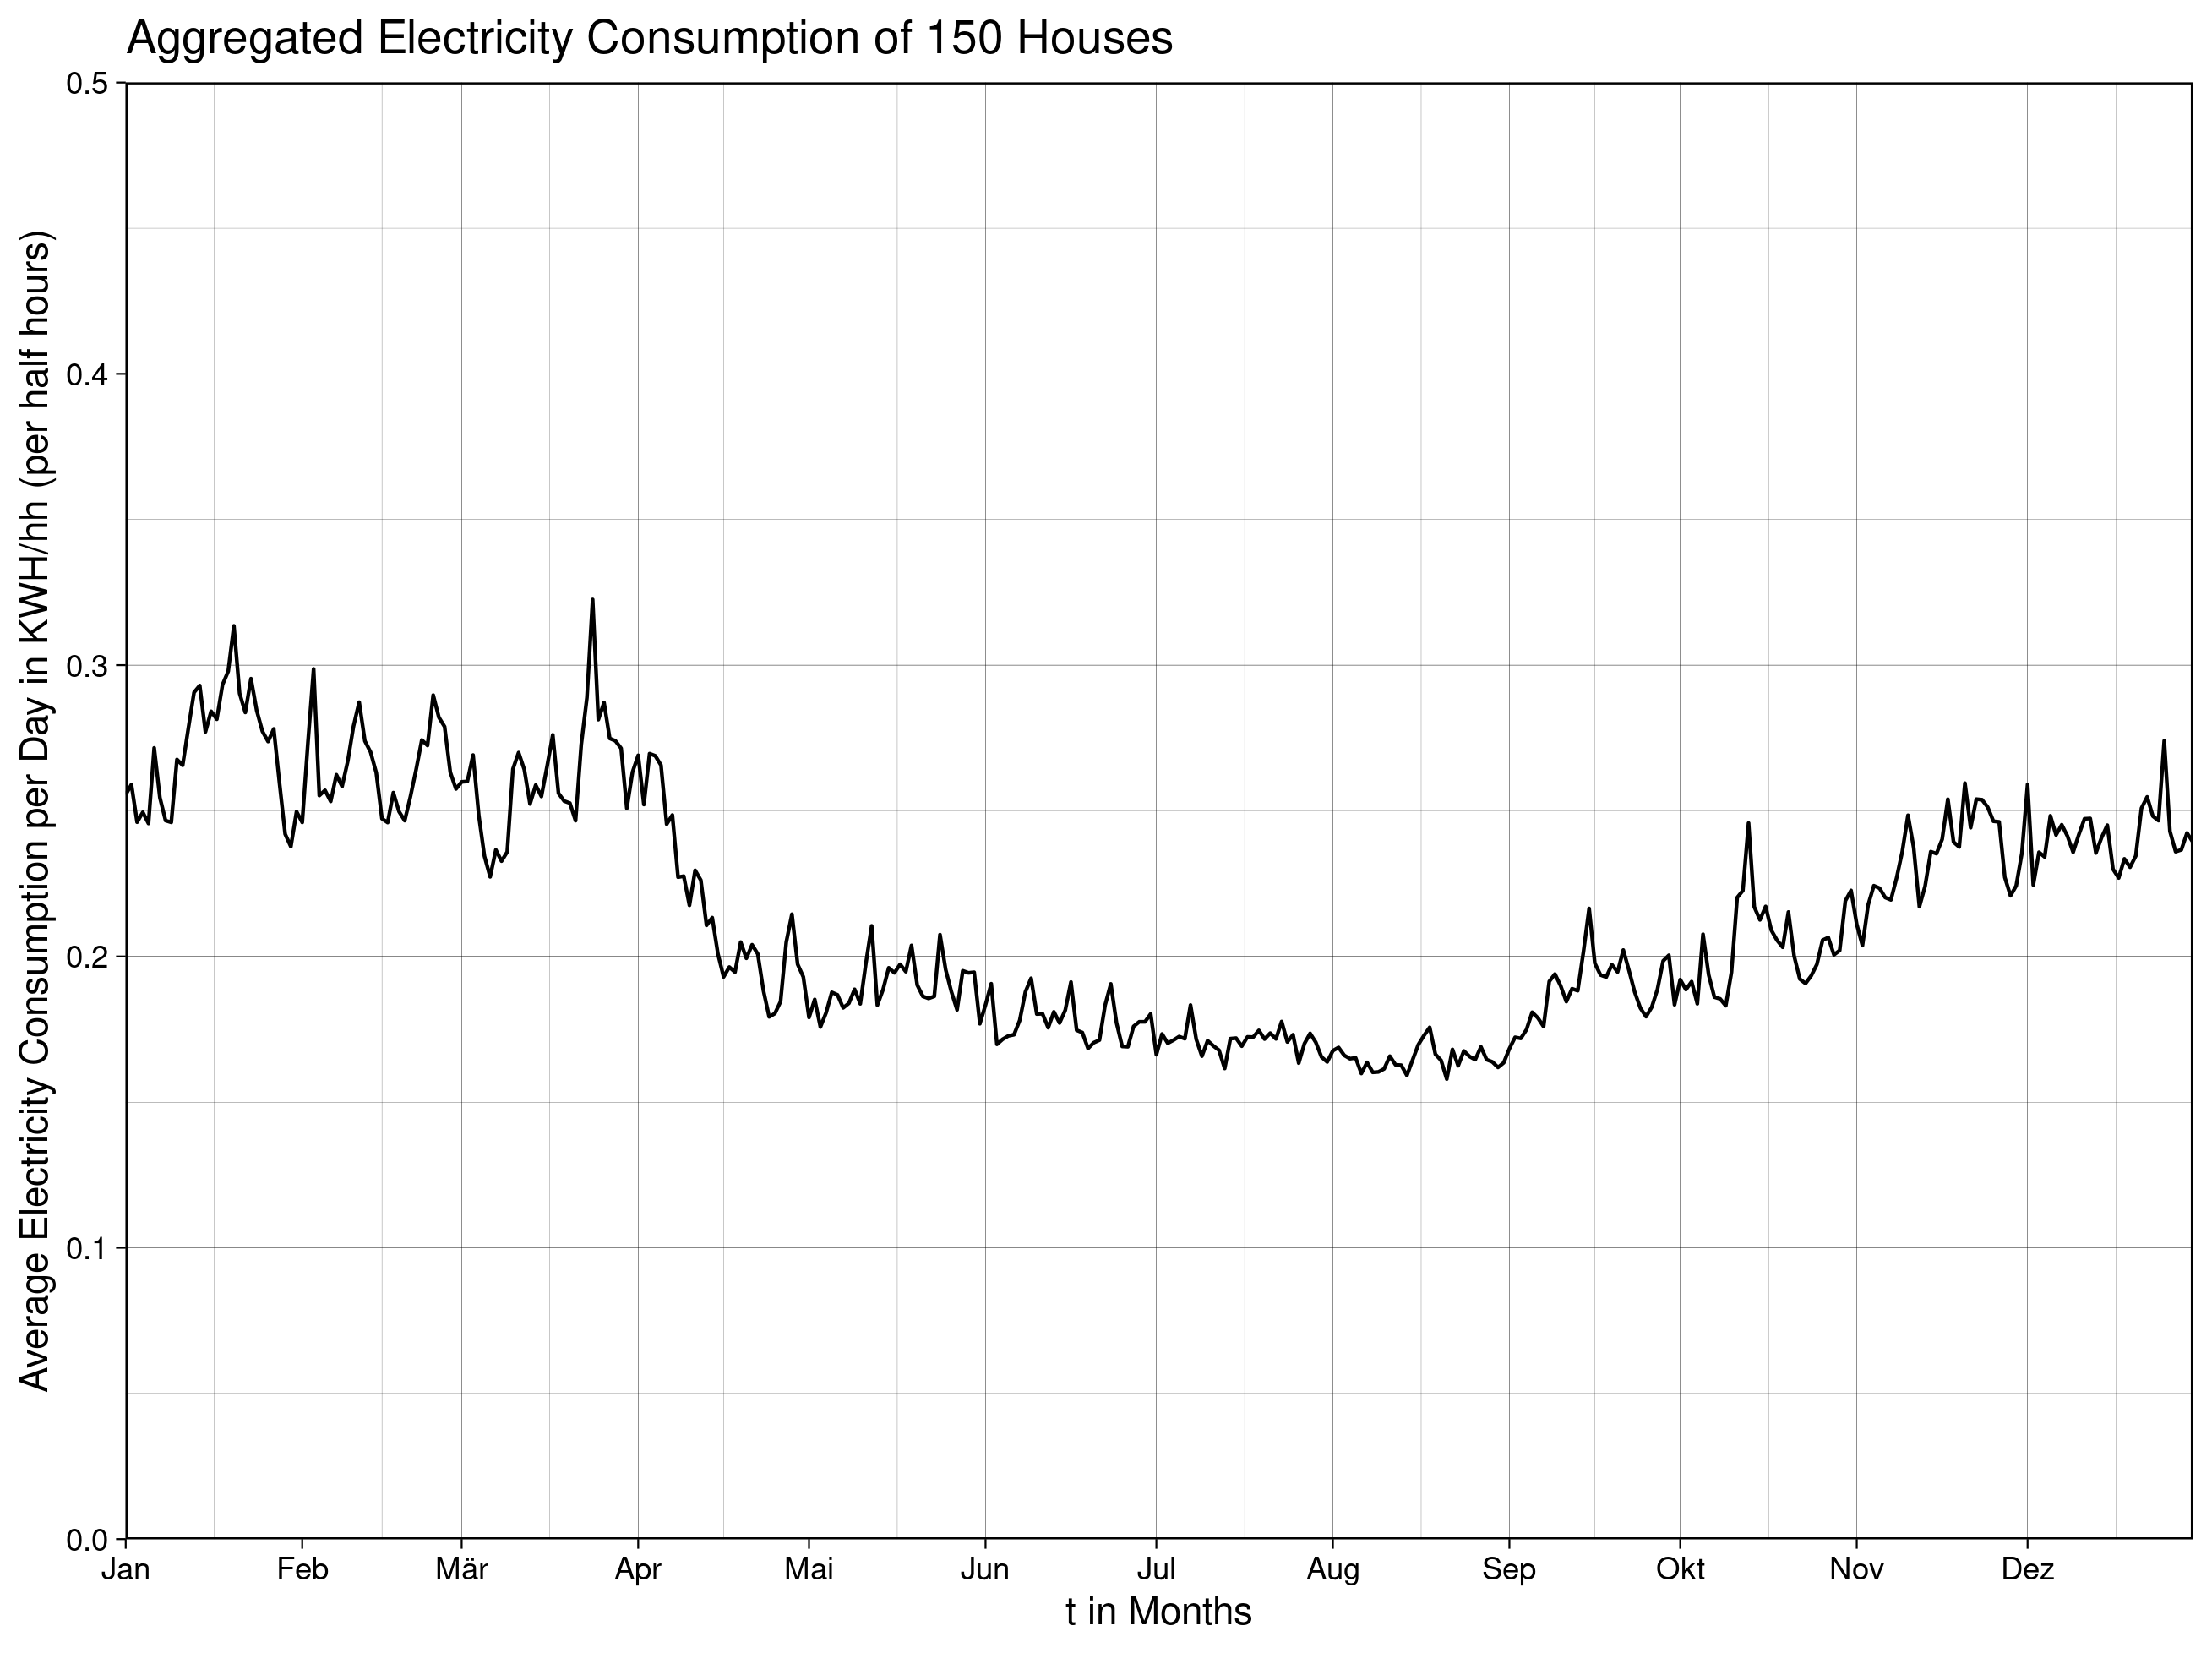
\includegraphics[width=0.85\textwidth]{images/Aggregated Electricity Consumption of 150 Houses.png}
\caption[Aggregated Electricity Consumption of 150 Houses]{}
\label{img:150_houses}
\end{figure}
\clearpage
}


\cleardoublepage

%%% Local Variables:
%%% TeX-master: "diplom"
%%% End:
